\nextslide{Basics}
\begin{enumerate}
\item{The Java Modelling Language (JML)}
\item{Jack}
\item{Coq}
\end{enumerate}

\nextslide{JML}\small
The {\purple Java Modelling Language} (JML)
is used to annotate the Java programs we want to verify with 
Jack.\\
%Jack use a {\purple weakest precondition calculus} to generate
%the proof obligations.\\
In JML you can express loop invariants, assertions method's
pre and post conditions.\\
JML has a really large syntax so every tool (except maybe JMLrac)
implements only a {\purple portion} of its syntax.
\nextslide{JML constructions used (1)}
\small
\blist
\item Expressions used in annotations are special {\purple boolean expressions}:
\blist
  \item $\backslash$forall
  \item $\backslash$exists
  \item $\backslash$old
  \item methods if they are pure
\elist
\item Methods:
  \blist 
  \item requires 
  \item ensures
  \item modifies
  \elist
\item Assertions with the {\purple assert} construct
\elist
\nextslide{JML constructions used (2)}
\small
\blist
\item Loop invariants, termination:
  \blist 
  \item loop\_invariant
  \item decreases
  \item \ {\purple loop\_modifies}
  \elist
\item ghost variables
  \blist
  \item ghost v;
  \item set v = value;
  \elist
\elist
\nextslide{Jack (1)}
\small
\blist
\item Programmed mainly by {\purple Lilian Burdy}
\item Uses a {\purple weakest precondition calculus} to generate proof obligations
\item The proof obligations are decomposed w.r.t. the different 
{\purple execution cases}
\elist
\begin{center}
\includegraphics[width= \linewidth]{jack.ps}
\end{center}
\nextslide{Jack (2)}
\small
\blist
\item At first single prover (B)
\item Multi-prover interface (Simplify, Coq, PVS)
\item Fully integrated in {\purple Eclipse} as a plugin, and use a 
{\purple plugin architecture} to include new provers
\item To prove the quicksort we used the {\purple Coq Output} from Jack
\item Coq plugin in can be both used to prove {\purple automatically and
interactively} the proof obligations generated by Jack
\elist

\nextslide{Coq}
\small
Coq is based on the {\purple calculus of inductive constructions}.\\
You can express: types, axioms, functions
variables, definitions, {\purple lemmas}...

Lemmas have to be proved.\\
To prove a lemma you have to build a {\purple proof term} out of the types, 
axioms, variables... \\
To build this proof term you use special commands 
called {\purple tactics} within a proof script.

{\purple Custom tactics} can be created composing more primitive ones.\\

It can easily express the logics for Jack.
\nextslide{Coq with Jack}
\small
The files generated by Jack in Coq can be separated into 3 categories:
\blist 
\item The {\purple prelude} containing the logic used :
\blist 
\item A static part (jack.arith.v jack.references.v jack.tactics.v)
\item A dynamic part generated for a specified class (myClass.classes.v 
myClass.subtypes.v myClass.v)

\elist
\item The {\purple proof obligation} (1 file)
\item A file containing some {\purple custom tactics} written by the user
\elist
To edit the files we use the {\purple CoqEditor} plugin, an integrated editor for Coq files in Eclipse.
